\chapter{Background}

\label{Chapter2}

\lhead{Chapter 2. \emph{Background}}

%----------------------------------------------------------------------------------------
%	Initial Approach
%----------------------------------------------------------------------------------------

\section{Initial Approach}

\subsection{Assessing Project Scope}
The first problem encountered immediately in my project was in specifying
specifically what problem I wanted to solve, and which direction I should take
my project in. The initial proposition by my supervisor was very broad, 
enabling me to look into a wide variety of goals. In particular, I saw two separate areas
of focus -- there was a clear divide between looking \emph{within} individual git 
projects and comparing statistics \emph{between} multiple projects, with both 
enabling interesting data to be gathered. 

The possibilities of looking within projects is quite exciting, as it could enable a solution
to a problem that appears fairly regularly in industry -- the handover problem \cite{handover}.
For example, if we were to provide information about certain files and even lines which are 
often modified in commits, it could highlight an area with a high potential for error.
Further to this, we could integrate the git commit analyses with a testing
framework, creating a tool to indicate good and bad coders -- those who add
tests, those who frequently break them etc.

There is also interesting potential in examining the data given between different
git projects. When we consider undergraduate work in earlier years, there are a
large number of courseworks which have the same specification, completed by 
individuals. This will allow us to directly compare statistics on these pieces
of work and gain some insight into the students' workflow, and even how this
compares to their grade received. Some areas of note in this area include comparing
areas of code modified, their start and end times, and the methodologies used
by undergraduates vs. postgraduates working on the same projects. The results
could easily be cross referenced against their grades to indicate successful
or poor approaches.

\subsection{Code Similarity}

I chose to look more closely at the problems surrounding the comparison of
multiple code repositories as this would open the door to building a tool which
could be of use to fellow students as they undertake programming exercises for
their studies. It's possible that a project in this area could also benefit lab
coordinators, aiding in marking and feedback. For example, following some of the
techniques mentioned above, an analysis of git habits could reveal important
correlations between grades and certain workflows which could aid feedback and teaching.

Taking the analysis further, I considered what other information we could gather
from multiple code bases. Given the students all work toward the same coursework
specification, and in many cases, even from the same skeleton files, it would be
interesting to see how their code itself is similar or different. In parsing
the students code and using a certain means to analyse it, there is a huge 
amount of analysis we could perform on the results. This would
deviate from the focus of version control, but could provide a wealth of 
information on the students' approach to exercises.

It is down this avenue that I felt investing my time would be most fruitful --
it would be very interesting to look into the similarities of student code,
possibly comparing the approach to the marks received. Students would be
able to look at this and see where they're particular approach differed
significantly from the top of the class' work (for example). We could also
highlight where a student came up with a particularly novel solution, if they
receive a high mark but with a low similarity to other pieces of work. This
would work well with a graphical representation of the code, as mocked up in
Figure \ref{fig:SimilarityVsGradeGraph}. Note the outlier, with a high grade but
low similarity, indicating a unique but good approach. It is also obvious how
this could be used to provide genericised feedback, for example ``everyone in
this cluster failed to spot the trick of calling function foo recursively''.

\begin{figure}[h!]
	\centering
		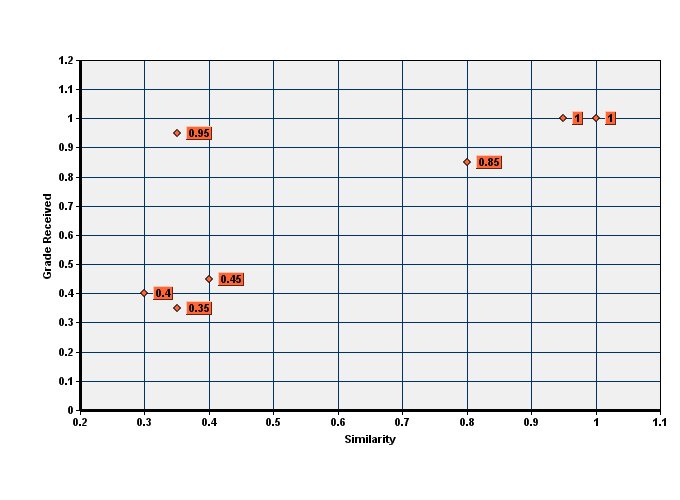
\includegraphics[width=\textwidth]{Figures/similarityVsGradeGraph}
	\caption{How a potential similarity graph may look, comparing each piece of
	code against the top graded work}
	\label{fig:SimilarityVsGradeGraph}
\end{figure}

I



%-----------------------------------
%	SUBSECTION 1
%-----------------------------------
\subsection{Subsection 1}


%----------------------------------------------------------------------------------------
%	SECTION 2
%----------------------------------------------------------------------------------------

\section{Areas of Research}

Having discussed ideas with my proejct supervisor, and feeling happy with the
focus on code similarity, I proceeded to research academic articles which could
provide me with ideas and techniques to use in my project. We agreed that the
techniques used in plagiarism detection would be beneficial here, as what I aim
to achieve is essentially a less strict plagiarism detector. i.e. rather than
looking for a binary answer, ``yes'' vs. ``no'', to the similarity of code, I'd
want to find how similar the code is.

The issue of code similarity is a complex one, and solutions to the problem
vary wildly in terms of technique, complexity and accuracy. Although plagiarism
detection in essays and other extended writing tasks has been 
researched by many and a large number of working products exist, the research
into plagiarism detection within code is still a largely changing area. There
is currently no established norm to follow in building our solution. Our problem
is exacerbated by the fact that, as previously touched upon,
any research into plagiarism detection is
generally looking for a solution which can output a binary result, whereas the
aim of this project is to produce an output which gives a sliding scale.

My initial searches pointed me in the direction of the MOSS plagiarism detection
system. MOSS is a popular tool used throughout academia for detecting plagiarism
in code, which accepts a large number of input source code files and uses certain
techniques to check for plagiarism. The technique used is known as 
``winnowing''\cite{winnowing}. This process takes ideas from earlier detection
techniques, such as \emph{k-grams}, and applies their own algorithms to indicate
code duplication. The winnowing algorithm works by hashing substrings of length
\emph{k} (the \emph{k-grams}) and moving through \emph{windows} of these hashes.
The winnowing step is the defined as: 
\begin{quote}In each window select the minimum hash value.
If there is more than one hash with the minimum value, select the rightmost
occurence. Now save all selected hashes as the fingerprints of the document.
\cite{winnowing}
\end{quote}

This process is undertaken after refactoring the code so that whitespace
has minimal effect and, if possible, variable renaming to normalised names.
The resulting fingerprints are then compared with the fingerprints of another
code base, with more hits indicating a larger likelihood of plagiarism.

We can see how this could be applicable for the uses of code similarity -- 




\section{Further Considerations}